\documentclass{article}

% if you need to pass options to natbib, use, e.g.:
% \PassOptionsToPackage{numbers, compress}{natbib}
% before loading nips_2018

% ready for submission
%\usepackage{nips_2018}

% to compile a preprint version, e.g., for submission to arXiv, add
% add the [preprint] option:
\usepackage[preprint]{nips_2018}

% to compile a camera-ready version, add the [final] option, e.g.:
% \usepackage[final]{nips_2018}

% to avoid loading the natbib package, add option nonatbib:
% \usepackage[nonatbib]{nips_2018}

\usepackage[utf8]{inputenc} % allow utf-8 input
\usepackage[T1]{fontenc}    % use 8-bit T1 fonts
\usepackage{hyperref}       % hyperlinks
\usepackage{url}            % simple URL typesetting
\usepackage{booktabs}       % professional-quality tables
\usepackage{amsfonts}       % blackboard math symbols
\usepackage{nicefrac}       % compact symbols for 1/2, etc.
\usepackage{microtype}      % microtypography
\usepackage[super]{nth}     % JK: for 1st-ing and 2nd-ing

\usepackage{graphicx}       % added by seth - image support
\graphicspath{ {./images/} }
\usepackage{soul}           % added by seth - remove before submission, provides highlighting support

\usepackage{hyperref}
\hypersetup{
    colorlinks=true,
    linkcolor=blue,
    filecolor=magenta,      
    urlcolor=blue,
}
 
\urlstyle{same}
\title{%
  Kung Faux Pandas \\
  \large Alternative Facts for Privacy Protection}

\author{
  James King, Seth Russell, Tellen D. Bennett, Debashis Ghosh\\
  Data Science to Patient Value (D2V)\\
  School of Medicine\\
  University of Colorado Anschutz Medical Campus\\
  Aurora, CO\\
  \texttt{\{james.king, seth.russell, tell.bennett, debashis.ghosh\}@ucdenver.edu}
  }

\date{May 2018}

\begin{document}

% Advice from Tell:  articulate the problem with evidence (i.e. papers)
%   Enable reproducibility - patient value, make process of replication easier
%   Time saving
%   legal risk (carrying data in laptops, etc)
%   Multiple comparison?
%   Educational data sets
%  Definition of :reproducibility 
%       reproducibilty - everything same - code, data, result
%       replicability - code same, new data, same result find Peng & Leek reference (also look at blog)
%   unit testing...
%   Proof of privacy guarantees?

\maketitle

\begin{abstract}
A description of an end-to-end system for easily generating faux-data which is statistically similar to given real data but does not contain sensitive personal information.  This system, which is publicly available \footnote{\url{https://github.com/CUD2V/kungfauxpandas}}, enables data to be distributed for reproducibility testing and other purposes while in full compliance with HIPAA and GDPR.
\end{abstract}


\section{Introduction}

The ability of independent investigators to verify results is perhaps \emph{the} most fundamental feature that separates science from other forms intellectual inquiry.  Unfortunately, the mechanisms of communicating scientific results have changed little since the age of enlightenment and are inadequate enabling reproducibility for some modern scientific endeavors such as machine learning.  Perhaps the most important impediment to reproducibility is the need to share data.  This has long been difficult in health care fields, but will presently become difficult for just about everyone.

There is a large body of published literature detailing methods for overcoming this difficulty via ``anonymizing'' and ``synthesising'' data \cite{patki_synthetic_2016, choi_generating_2017}, however at present a mechanism to routinely \emph{use} these techniques has not been forthcoming.

This paper details an open source software library called \emph{Kung Faux Pandas (KFP)} which integrates \emph{any} of these data security methods into the popular Python Pandas data science library. For those who prefer other tools, KFP also provides Structured Query Language (SQL) interface which enables users to arbitrarily query any data within a database, returning to the user a data set which either does not contain any personal information (synthesized) or has been anonymized by standard methods.

\section{Background}

In the United States, there's been a long-standing regulation described in the Health Insurance Portability and Accountability Act (HIPAA), which mandates strong security on data related to health care and is backed by significant fines and possible criminal charges \cite{hippaviol}.  Thus, even institutions which share data face a steep institutional risk. This makes it virtually impossible to enable independent verification of machine learning (ML) models which often require enormous amounts of training data.

Perhaps more ominously for researchers, on May 25 , 2018, the European Union's (EU) General Data Protection Regulation (GDPR) has come into full effect \cite{gdpr}, establishing a new paradigm in data ``ownership'' for that jurisdiction.   In short, this set of rules defines the ``owners'' of data to be people from whom it was collected and obliges anyone possessing  that data to  honor the owners' preferences about how the data is kept and used, including a requirement to deletion of any data at the request of its owner at any time in the future.

These rules are ultimately good for citizens, but they create a pickle for scientists studying humans as it's very difficult to follow normal processes in scientific rigor while complying with privacy protection rules.

One obvious way around this pickle is to separate data and analysis in such a way that the analysis can be performed on data without the \emph{analyst} having access to the data.   This is fairly straight-forward to implement.   Essentially, the analyst, with only a description of the sensitive data, composes analytical code which is handed off to the data custodian.  The custodian then runs it and returns the results to the researcher.

This has been technologically possible for some time, but it's awkward in practice because activities such as data cleaning, exploration, and plotting are interactive and iterative processes which would become impractical with a mediator.

Kung Faux Pandas sidesteps this problem by generating \emph{faux-data} that is ``statistically similar'' to the real data but does not itself contain any sensitive data.

This faux-data can be prodded, poked, plotted, and posted for the world to see, enabling analysts to develop their code using whatever means they prefer.   When the analytical code is ready, it can then be sent to the data custodian to run on the real data.


\section{System Details}

Many methods of generating the faux-data exist in the literature, many of which have software implementations freely available.   KFP provides a standard mechanism for ``wrapping'' any method into a ``plug-in'' which integrates the method with the Pandas data frame model.  Three of these plug-ins are provided with full documentation for creating other plug-ins.


\subsection{Included Methods}

\begin{tabular}{c c c p{7em}}


Method & Source & Plug-In Name & Notes \\ 
\hline 

Kernel Density\\Estimator & scipy.stats.gaussian\_kde & KDEPlugin & Useful for inter-related ordinal and ratio data \\ 

DataSynthesizer & Ping et al. & DataSynthesizerPlugin & Generates a Bayesian tree to capture column relationships \\ 

Synthetic dataset\\Generation Framework & Bindschaedler et al.  & SGFPlugin & Fast \\ 

\hline 
\end{tabular}

Some text~\ref{included-methods}

\begin{table}
  \caption{Kung Faux Pandas Data Synthesis Methods}
  \label{included-methods}
  \centering
  \begin{tabular}{llll}
    \toprule
    Method                                 & Source                    & Notes \\
    \midrule
    Kernel Density Estimator               & scipy.stats.gaussian\_kde & Inter-related ordinal and ratio data\\
    DataSynthesizer                        & Ping et al.               & Bayesian modeling of column relationships\\
    Synthetic dataset Generation\\Framework & Bindschaedler et al.     &  \\
    \bottomrule
  \end{tabular}
\end{table}

After table


\subsection{System Structure}
KFP provides a class

Describe KFP's structure, including the ``plugin'' mechanism.

Describe the SQL interface

Diagrams - not sure if we need both of these. Should we include a screenshot of the UI (saved to /images)?

\begin{figure}[h]
  \centering
  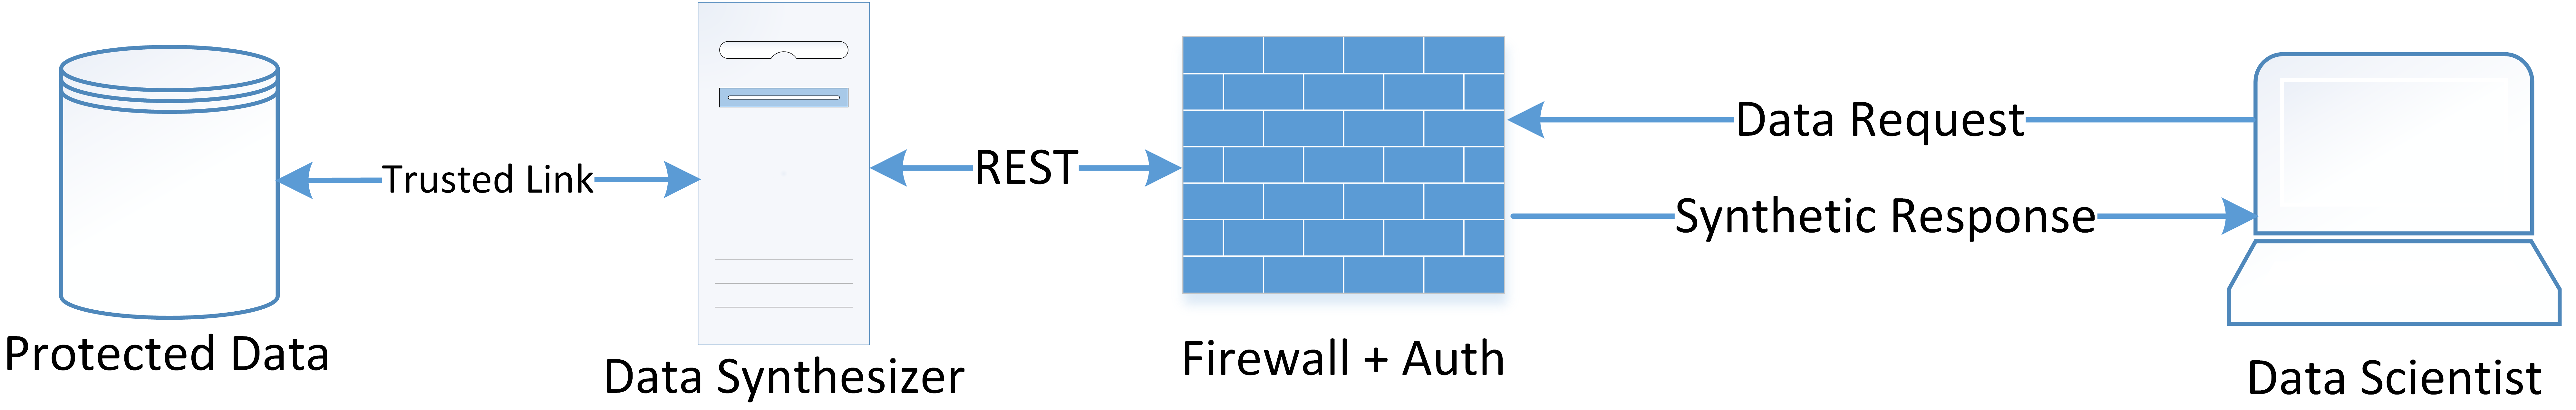
\includegraphics[width=\textwidth]{prototype_architecture}
  \caption{System Architecture.}
\end{figure}

\begin{figure}[h]
  \centering
  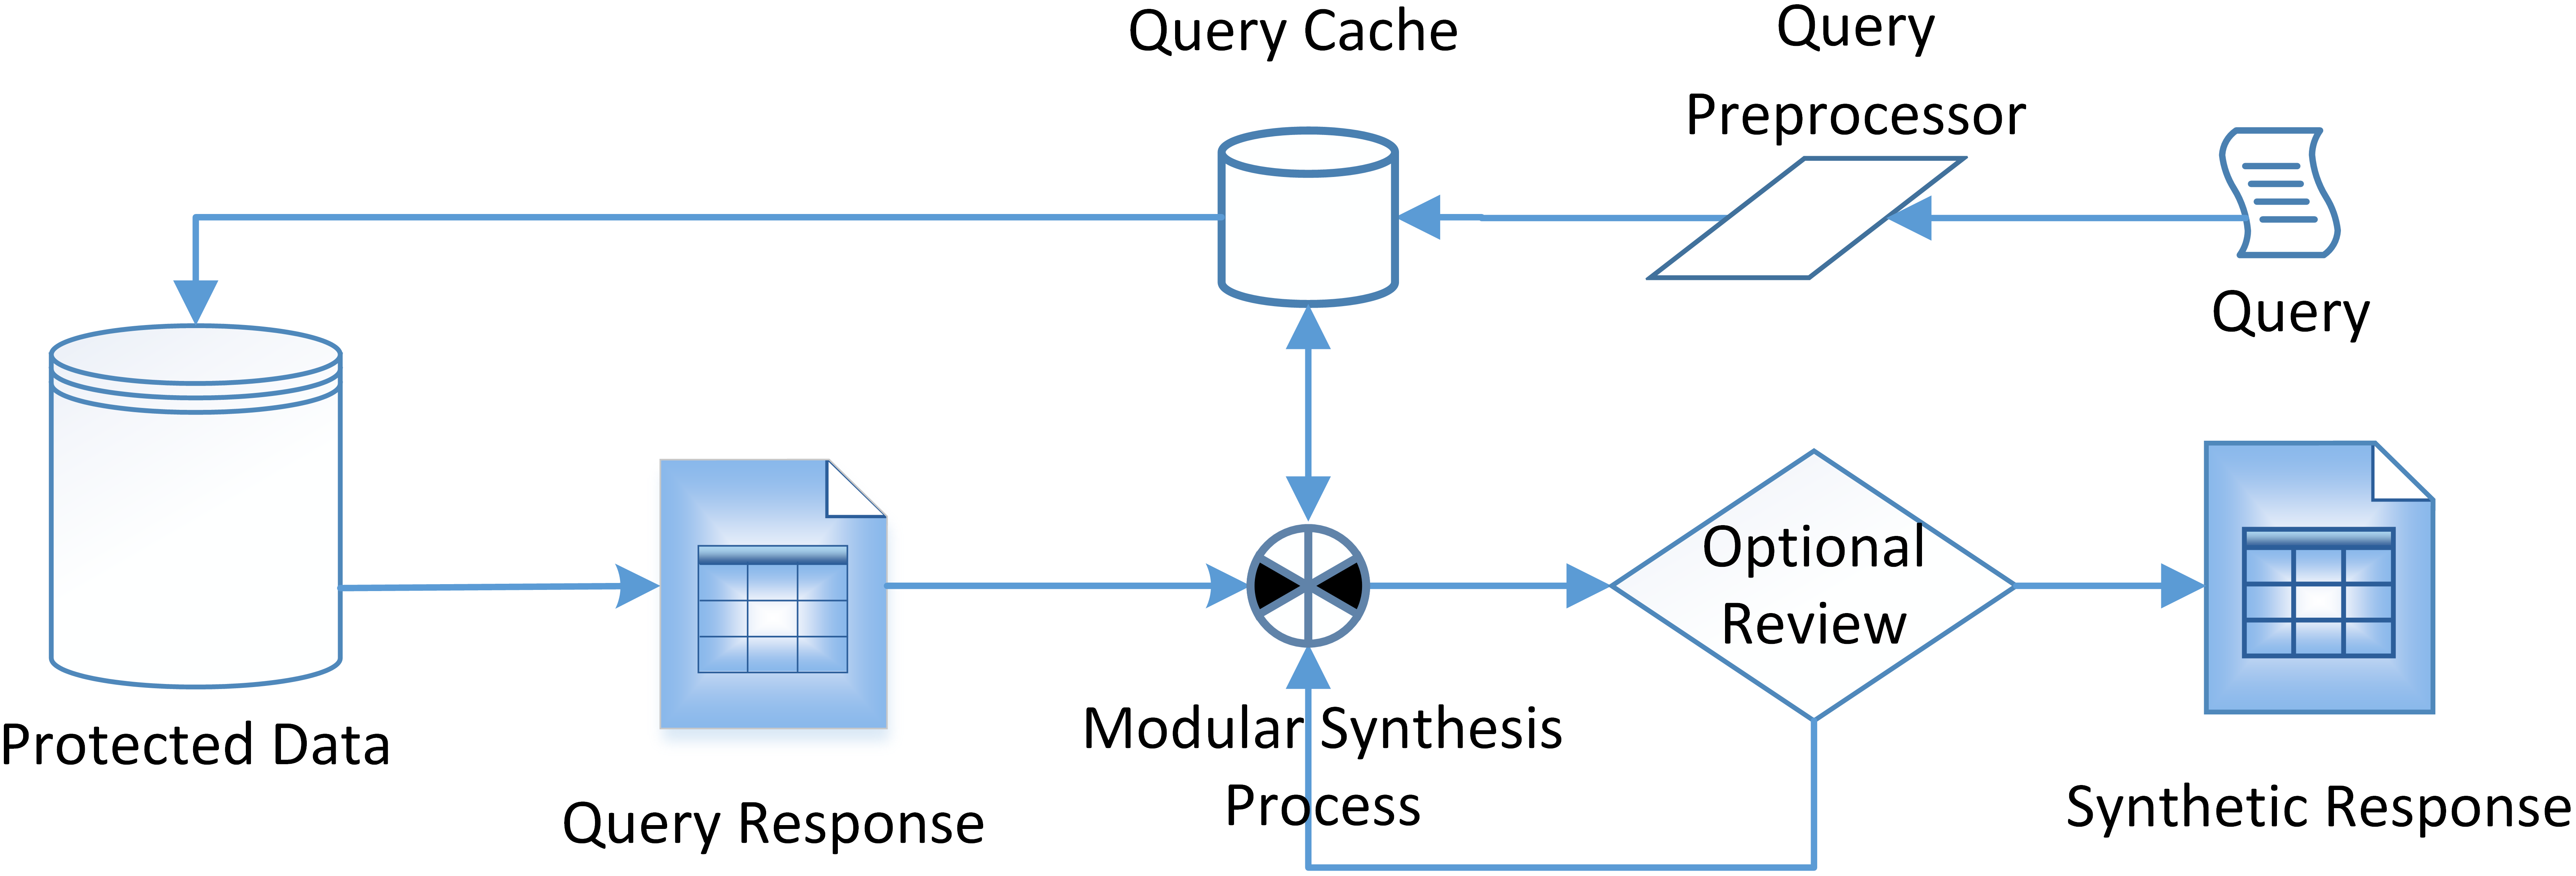
\includegraphics[width=115mm]{data_synthesis_process}
  \caption{Data synthesis process.}
\end{figure}


\section{Conclusion}

Basically need to put abstract here...


\bibliographystyle{unsrt}

\bibliography{bib}

\end{document}